\documentclass{article}

\usepackage{graphicx}
\usepackage{tikz}
\usepackage{tikzsymbols}
\usetikzlibrary{calc,patterns,shapes.geometric}
\pagestyle{empty}
\usepackage[margin=0pt]{geometry}
\geometry{papersize={14in,12in}}

\def\centerarc[#1](#2)(#3:#4:#5){\draw[#1] ($(#2)+({#5*cos(#3)},{#5*sin(#3)})$) arc (#3:#4:#5);}

\begin{document}
	\begin{figure}
		\centering
		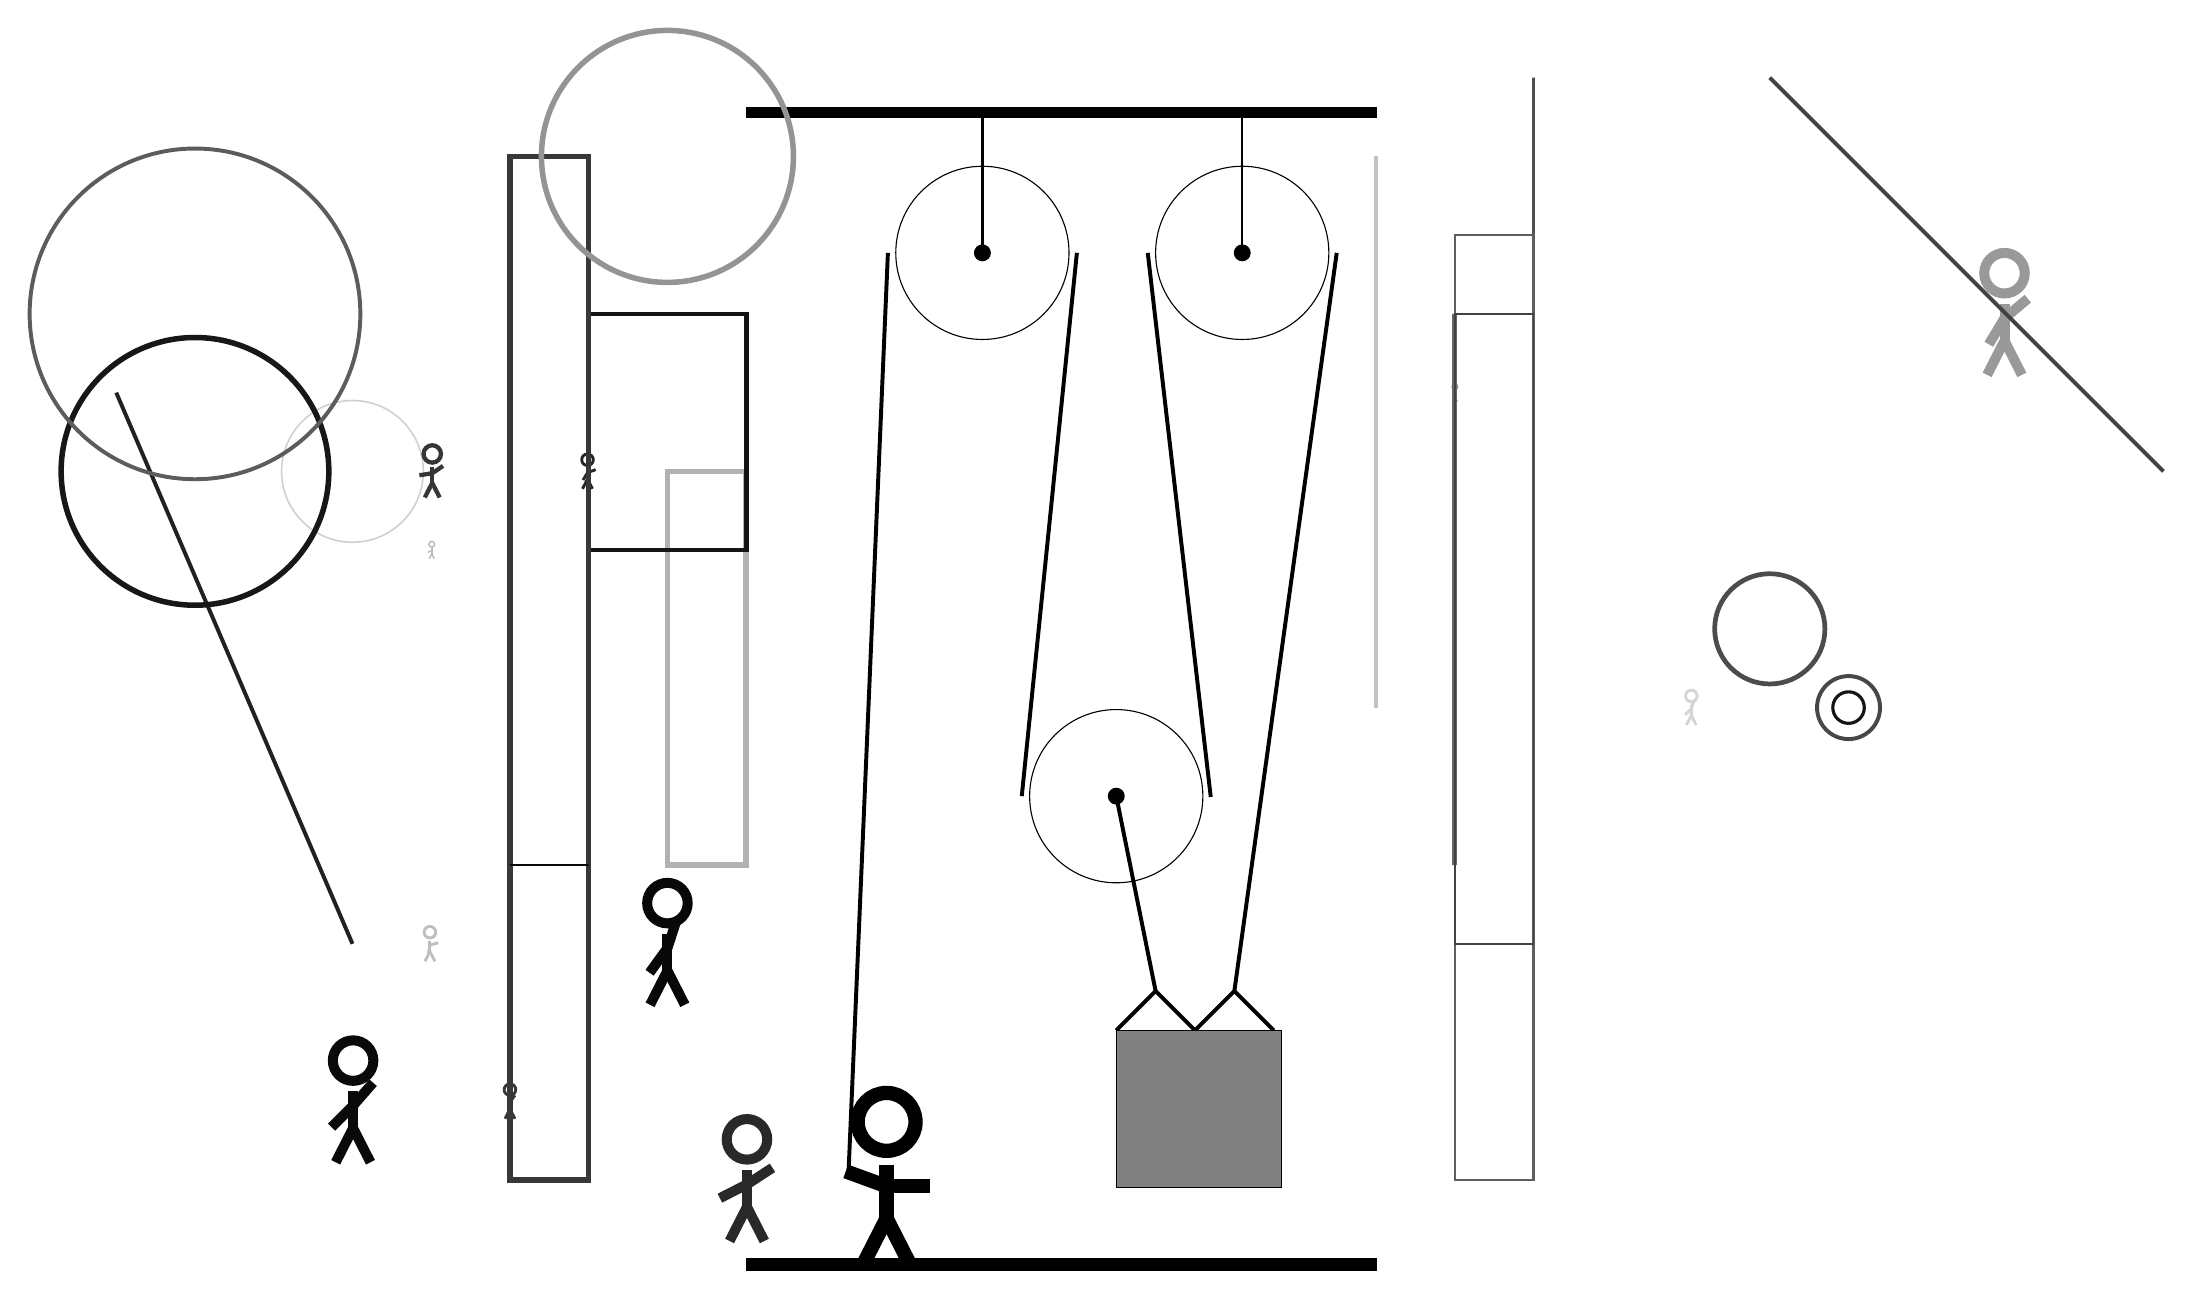
\begin{tikzpicture}
			%%%%% START %%%%%
			
			\draw[fill=black] (-2, 11.5) rectangle (6, 11.625);
			
			\draw (1, 9.775) circle (1.1);
			\draw[fill=black] (1, 9.775) circle (0.1);
			\draw[thick] (1, 9.775) -- (1, 11.5);
			
			\draw (4.3, 9.775) circle (1.1);
			\draw[fill=black] (4.3, 9.775) circle (0.1);
			\draw[thick] (4.3, 9.775) -- (4.3, 11.5);
			
			\draw (2.7, 2.875) circle (1.1);
			\draw[fill=black] (2.7, 2.875) circle (0.1);
			
			\draw[line width=0.5mm]  (2.7, -0.1) -- (3.2, 0.4) -- (3.7, -0.1) -- (4.2, 0.4) -- (4.7, -0.1);
			\draw[fill=black!50] (2.7, -0.1) rectangle (4.8, -2.1);
			
			\draw[line width=0.5mm](-0.7, -1.9) -- (-0.2, 9.775);
			\centerarc[line width=0.5mm](1, 9.775)(0:180:1.2000000000000002);
			\draw[line width=0.5mm](2.2, 9.775) -- (1.5, 2.875);
			\centerarc[line width=0.5mm](2.7, 2.875)(180:370:1.2000000000000002);
			\draw[line width=0.5mm] (3.9, 2.865) -- (3.1, 9.775);
			\centerarc[line width=0.5mm](4.3, 9.775)(0:180:1.2000000000000002);
			\draw[line width=0.5mm](4.2, 0.4) -- (5.5, 9.775);
			\draw[line width=0.5mm] (3.2, 0.4) -- (2.7, 2.875);
			
			\node[line width=0.3mm, color=black!86] at (-4, 7) {\Strichmaxerl[2][59][20]};
			
			\draw [line width=0.5mm, color=black!72](12, 4) circle (0.4);
			\node[line width=0.2mm, color=black!25] at (-6, 1) {\Strichmaxerl[2][80][15]};
			\node[line width=0.5mm, color=black!40] at (14, 9) {\Strichmaxerl[7][59][40]};
			\node[line width=0.7mm, color=black!96] at (-7, -1) {\Strichmaxerl[7][45][49]};
			\node[line width=0.2mm, color=black!39] at (7, 8) {\Strichmaxerl[1][62][70]};
			
			\draw[line width=0.7mm, color=black!30] (-2, 7) rectangle (-3, 2);
			
			\node[line width=0.5mm, color=black!79] at (-5, -1) {\Strichmaxerl[2][90][56]};
			\node[line width=0.6mm, color=black!27] at (-6, 6) {\Strichmaxerl[1][21][82]};
			\draw[line width=0.3mm, color=black!69] (8, 10) rectangle (8, 12);
			\draw[line width=0.6mm, color=black!92] (-2, 9) rectangle (-4, 6);
			\draw[line width=0.7mm, color=black!78] (-4, 11) rectangle (-5, -2);
			\draw[line width=0.5mm, color=black!87](-7, 1) -- (-10, 8);
			
			\draw [line width=0.2mm, color=black!19](-7, 7) circle (0.9);
			\draw[line width=0.5mm, color=black!24](6, 4) -- (6, 11);
			\draw [line width=0.6mm, color=black!70](11, 5) circle (0.7);
			\draw[line width=0.3mm, color=black!63] (7, -2) rectangle (8, 10);
			
			\draw [line width=0.4mm, color=black!92](12, 4) circle (0.2);
			\draw[line width=0.5mm, color=black!74](11, 12) -- (16, 7);
			
			\draw[line width=0.2mm, color=black!97] (-4, 2) rectangle (-5, 2);
			\draw [line width=0.7mm, color=black!42](-3, 11) circle (1.6);
			
			\draw[line width=0.6mm, color=black!60] (7, 9) rectangle (7, 2);
			\node[line width=0.5mm, color=black!97] at (-3, 1) {\Strichmaxerl[7][54][72]};
			\node[line width=0.4mm, color=black!79] at (-6, 7) {\Strichmaxerl[3][9][34]};
			\draw [line width=0.7mm, color=black!91](-9, 7) circle (1.7);
			\draw[line width=0.2mm, color=black!74] (8, 9) rectangle (7, 1);
			\node[line width=0.5mm, color=black!84] at (-2, -2) {\Strichmaxerl[7][27][33]};
			\draw [line width=0.5mm, color=black!64](-9, 9) circle (2.1);
			\node[line width=0.5mm, color=black!17] at (10, 4) {\Strichmaxerl[2][44][72]};
			
			\node at (-0.2, -2) {\Strichmaxerl[10][-20][0]};
			
			\draw[fill=black] (-2, -3) rectangle (6, -3.15);
			
			%%%%% END %%%%%
		\end{tikzpicture}
	\end{figure}	
\end{document}